\PassOptionsToPackage{unicode=true}{hyperref} % options for packages loaded elsewhere
\PassOptionsToPackage{hyphens}{url}
%
\documentclass[]{article}
\usepackage{lmodern}
\usepackage{amssymb,amsmath}
\usepackage{ifxetex,ifluatex}
\usepackage{fixltx2e} % provides \textsubscript
\ifnum 0\ifxetex 1\fi\ifluatex 1\fi=0 % if pdftex
  \usepackage[T1]{fontenc}
  \usepackage[utf8]{inputenc}
  \usepackage{textcomp} % provides euro and other symbols
\else % if luatex or xelatex
  \usepackage{unicode-math}
  \defaultfontfeatures{Ligatures=TeX,Scale=MatchLowercase}
\fi
% use upquote if available, for straight quotes in verbatim environments
\IfFileExists{upquote.sty}{\usepackage{upquote}}{}
% use microtype if available
\IfFileExists{microtype.sty}{%
\usepackage[]{microtype}
\UseMicrotypeSet[protrusion]{basicmath} % disable protrusion for tt fonts
}{}
\IfFileExists{parskip.sty}{%
\usepackage{parskip}
}{% else
\setlength{\parindent}{0pt}
\setlength{\parskip}{6pt plus 2pt minus 1pt}
}
\usepackage{hyperref}
\hypersetup{
            pdfborder={0 0 0},
            breaklinks=true}
\urlstyle{same}  % don't use monospace font for urls
\usepackage{graphicx,grffile}
\makeatletter
\def\maxwidth{\ifdim\Gin@nat@width>\linewidth\linewidth\else\Gin@nat@width\fi}
\def\maxheight{\ifdim\Gin@nat@height>\textheight\textheight\else\Gin@nat@height\fi}
\makeatother
% Scale images if necessary, so that they will not overflow the page
% margins by default, and it is still possible to overwrite the defaults
% using explicit options in \includegraphics[width, height, ...]{}
\setkeys{Gin}{width=\maxwidth,height=\maxheight,keepaspectratio}
\setlength{\emergencystretch}{3em}  % prevent overfull lines
\providecommand{\tightlist}{%
  \setlength{\itemsep}{0pt}\setlength{\parskip}{0pt}}
\setcounter{secnumdepth}{0}
% Redefines (sub)paragraphs to behave more like sections
\ifx\paragraph\undefined\else
\let\oldparagraph\paragraph
\renewcommand{\paragraph}[1]{\oldparagraph{#1}\mbox{}}
\fi
\ifx\subparagraph\undefined\else
\let\oldsubparagraph\subparagraph
\renewcommand{\subparagraph}[1]{\oldsubparagraph{#1}\mbox{}}
\fi

% set default figure placement to htbp
\makeatletter
\def\fps@figure{htbp}
\makeatother


\date{}

\begin{document}

\hypertarget{questions}{%
\section{Questions}\label{questions}}

\hypertarget{one}{%
\subsection{One}\label{one}}

\hypertarget{lewis-structure-of-sioh_4}{%
\subsubsection{\texorpdfstring{Lewis structure of
\(Si(OH)_4\)}{Lewis structure of Si(OH)\_4}}\label{lewis-structure-of-sioh_4}}

,\_

\hypertarget{step-1}{%
\paragraph{Step \#1}\label{step-1}}

Number of electrons = 4x6 +4x1 +1x4 = 32.

\hypertarget{step-2}{%
\paragraph{Step \#2}\label{step-2}}

After 8 electrons are assigned to each oxygen, and single bonds are
formed between each species all species have a full octet, (except for
hydrogen which has a full valence shell consisting of two electrons)

NOTE: As silica is a period two element overfilling of the octet is
possible however any additional bond formation between the oxygen and
the central silicon could only increase the formal charge and so may be
discounted.

\hypertarget{step-3}{%
\paragraph{Step \#3}\label{step-3}}

Draw structure

\begin{figure}
\centering
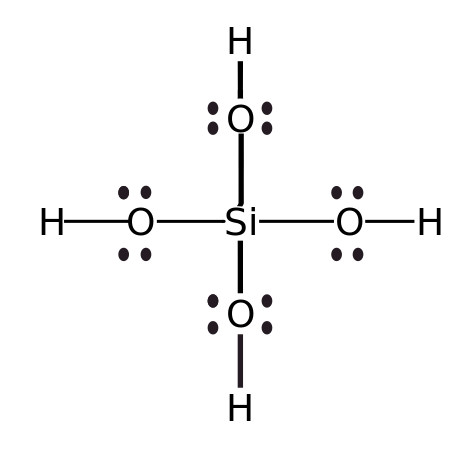
\includegraphics[width=0.5\textwidth,height=\textheight]{Images/SiliconHydroxideLewisStructure.jpg}
\caption{Silicon Hydroxide Lewis structure}
\end{figure}

\hypertarget{lewis-structure-of-aloh_4--}{%
\subsubsection{\texorpdfstring{Lewis structure of
\(Al(OH)_4 ^{-}\)}{Lewis structure of Al(OH)\_4 \^{}\{-\}}}\label{lewis-structure-of-aloh_4--}}

,\_

\hypertarget{step-1-1}{%
\paragraph{Step \#1}\label{step-1-1}}

Number of electrons = 4x6 +4x1 +1x3+1 = 32.

\hypertarget{step-2-1}{%
\paragraph{Step \#2}\label{step-2-1}}

After 8 electrons are assigned to each oxygen, and single bonds are
formed between each species all species have a full octet, (except for
hydrogen which has a full valence shell consisting of two electrons).
Again overfilling by creating more bonds will only increase the formal
charge.

\hypertarget{step-3-1}{%
\paragraph{Step \#3}\label{step-3-1}}

Draw Structure

\begin{figure}
\centering
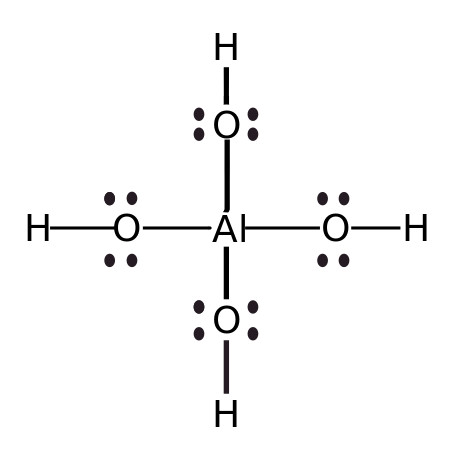
\includegraphics[width=0.5\textwidth,height=\textheight]{Images/AluminiumHydroxideIonLewisStructure.jpg}
\caption{Aluminium Hydroxide Ion Lewis structure}
\end{figure}

\hypertarget{lewis-structure-of-aloh_3}{%
\subsubsection{\texorpdfstring{Lewis Structure of
\(Al(OH)_3\)}{Lewis Structure of Al(OH)\_3}}\label{lewis-structure-of-aloh_3}}

,\_

\hypertarget{step-1-2}{%
\paragraph{Step \#1}\label{step-1-2}}

Number of electrons = 3x6 +3x1 +1x3= 32

\hypertarget{step-2-2}{%
\paragraph{Step \#2}\label{step-2-2}}

After 8 electrons are assigned to each oxygen, and single bonds are
formed between each species all species have a full octet, (except for
hydrogen which has a full valence shell consisting of two electrons).
Again overfilling by creating more bonds will only increase the formal
charge.

\hypertarget{step-3-2}{%
\paragraph{Step \#3}\label{step-3-2}}

Draw Structure

\begin{figure}
\centering
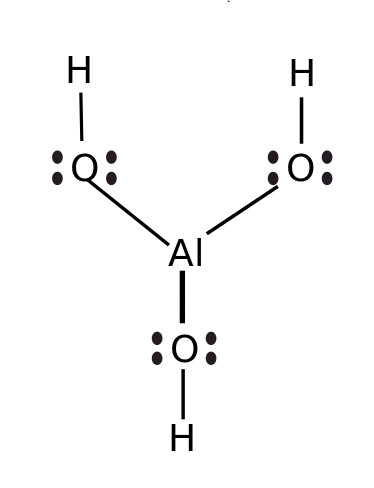
\includegraphics[width=0.5\textwidth,height=\textheight]{Images/AluminiumHydroxideLewisStructure.jpg}
\caption{Aluminium Hydroxide Ion Lewis structure}
\end{figure}

\hypertarget{two}{%
\subsection{Two}\label{two}}

\hypertarget{i}{%
\subsubsection{(i)}\label{i}}

\hypertarget{step-1-3}{%
\paragraph{Step \#1}\label{step-1-3}}

Moles of EDTA added to EDTA standard

\(= \frac{0.914g}{372.24g.mol^{-1}}\)
\(= 2.4554 \quad x \quad 10^{-3}mol\)

\hypertarget{step-2-3}{%
\paragraph{Step \#2}\label{step-2-3}}

Average Titrant volume \(= 0.5x ((4.57-0.04)+(5.13-0.10))ml= 4.78ml\)

\hypertarget{step-3-3}{%
\paragraph{Step \#3}\label{step-3-3}}

Moles of EDTA in Titrant

\(= 2.4554 \quad x \quad 10^{-3}mol \quad x \quad \frac{4.78ml}{250ml}\)

\(= 4.6947 \quad x \quad 10^{-5}mol\)

\hypertarget{ii}{%
\subsubsection{(ii)}\label{ii}}

\hypertarget{step-1-4}{%
\paragraph{Step \#1}\label{step-1-4}}

At equivalence point of the titration all of the EDTA has reacted with
calcium at the ratio of 1 mol EDTA: 1 mol calcium ions.

Hence If \(= 4.6947 \quad x \quad 10^{-5}mol\) of calcium where added
then \(= 4.6947 \quad x \quad 10^{-5}mol\) of calcium ions where used up
form the titrand.

\hypertarget{step-2-4}{%
\paragraph{Step \#2}\label{step-2-4}}

As the titrand contained only 25ml of the original calcium chloride
zeolite solution, It can be interpolated that
\(3 \quad x\quad 4.6947 \quad x \quad 10^{-5}mol= 1.4084 \quad x \quad 10^{-4}\)\\
of calcium ions would have been used up from the entire solution.

\hypertarget{iii}{%
\subsubsection{(iii)}\label{iii}}

\hypertarget{step-1-5}{%
\paragraph{Step \#1}\label{step-1-5}}

Moles of Calcium chloride present in the original solution.

\(\quad = \frac{0.196g}{219.08g.mol^{-1}}\)

\(\quad = 8.9465 \quad x \quad 10{-4}\)

\hypertarget{step-3-4}{%
\paragraph{Step \#3}\label{step-3-4}}

Moles of Calcium ions left in the original solution

\(\quad = 8.9465 \quad x \quad 10^{-4}mol - 1.4084 \quad x \quad 10^{-4}mol\)

\(\quad 7.5381 x \quad 10^{-4}mol\)

\hypertarget{iv}{%
\subsubsection{(iv)}\label{iv}}

Grams of Calcium chloride left in original solution.
\(\quad = 7.5381 x \quad 10^{-4}mol \quad x \quad 40.08g.mol^{-1}\)
\(\quad = 3.0213 \quad x \quad 10^{-2}g\)

\hypertarget{v}{%
\subsubsection{(v)}\label{v}}

\hypertarget{step-1-6}{%
\paragraph{Step \#1}\label{step-1-6}}

The amount of calcium ions taken up by the zeolite is equivalent to the
amount fo calcium ions remaining in solution, as any calcium ions not
bound would have been removed during the EDTA titration.

Hence there are \(7.5381 \quad x \quad 10^{-4}mol\) of Calcium ions
bound by the zeolite.

\hypertarget{vi}{%
\subsubsection{(vi)}\label{vi}}

\hypertarget{step-1-7}{%
\paragraph{Step \#1}\label{step-1-7}}

Grams of Calcium ions taken up per gram of Zeolite

\(\quad = \frac{3.0213 \quad x \quad 10^{-2}g}{0.104g}\)

\(\quad = 0.29051 (g/g)\)

\hypertarget{three}{%
\subsection{Three}\label{three}}

This implies that zeolites may be very useful as detergents as they are
capable of sequestering/removing relatively large quantities of
dissolved ions from solution. (removing these ions will prevent them
from resettling on whatever item is being cleaned, and increase the
overall ability of the detergent to dissolve and remove unwanted
deposits from the item being cleaned.)

\hypertarget{five}{%
\subsection{Five}\label{five}}

four acid sites are accosted with the EDTA. (one for each of the
terminal carboxylic acid groups)

\hypertarget{six.}{%
\subsection{Six.}\label{six.}}

Yes. Sulphuric acid has the same activity of any normal acid catalyst,
providing a ready source and sink for \(H^{+}\) ions, facilitating the
internal structural changes necessary for ester formation.

\hypertarget{seven}{%
\subsection{Seven}\label{seven}}

Pentyl ethanol is used:

\begin{enumerate}
\def\labelenumi{\arabic{enumi}.}
\item
  as a flavourant in many foods.
\item
  As a solvent in paints.
\end{enumerate}

\hypertarget{eight}{%
\subsection{Eight}\label{eight}}

Zeolite is micro-porous, that is within its 3D chemical structure there
is a regular arrangement of regular sized gaps/holes/pores,through which
other molecules, if sufficiently small could pass through. molecules
which are too large however, (such as molecules with a diameter greater
than X in the figure below) can. Such molecules suffer size exclusion,
as although they may have the correct chemical properties to react with
binding sites on the interior, they are physically prevented from
reaching these sites, as the are too large, and so cannot bind.

\begin{figure}
\centering
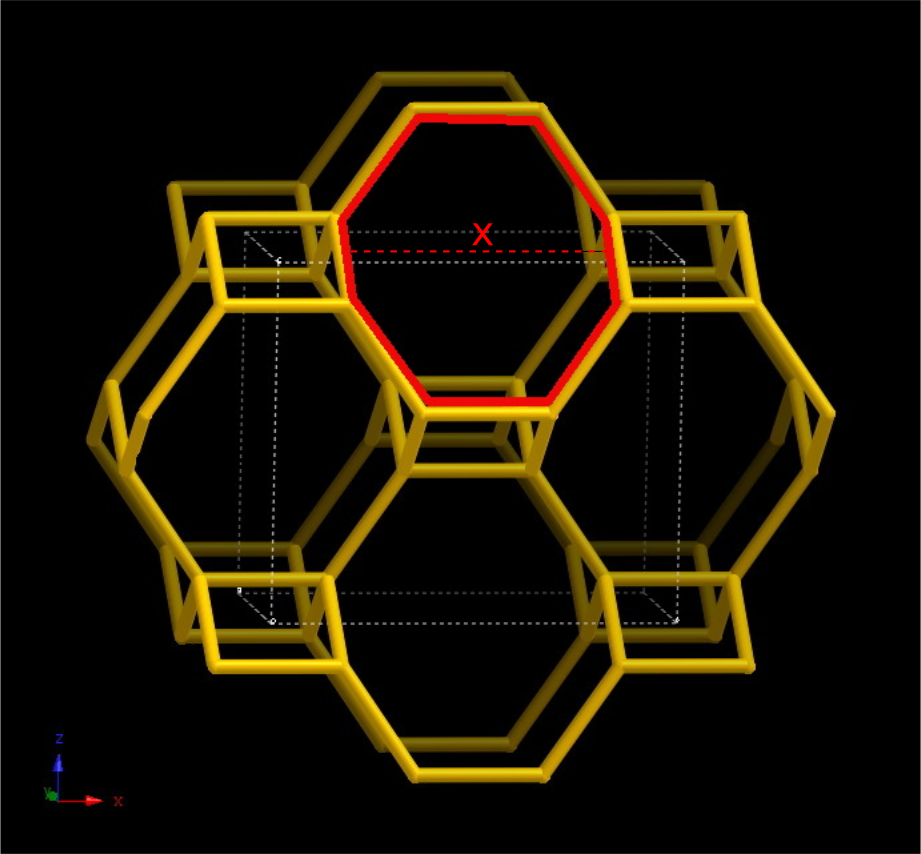
\includegraphics[width=0.5\textwidth,height=\textheight]{Images/ZeoliteStructure2.jpg}
\caption{Zeolite Structure}
\end{figure}

\hypertarget{aim}{%
\section{Aim}\label{aim}}

Two different experiments where performed with different aims.

The aim of experiment A was to determine the Ability of Zeolite to bind
Calcium ions from solution. Both to determine how effective Zeolite
could be as a cleaning/filtering agent to remove calcium impurities, and
to approximate how much zeolite (by mass) would be necessary to remove
calcium from a contaminated solution.

The aim of experiment B was to determine Zeolite ability to act as a
Acid catalyst (in esterification.)

\hypertarget{introduction}{%
\section{Introduction}\label{introduction}}

Zeolites Are complex three dimensional molecules formed from the
condensation of \$Si(OH)\emph{\{4\} \$} and \(Ai(OH)^{-}_{4}\)
monomers.The striking feature of the complexes formed are the regularly
sized and evenly space pores which the macro structure contains, (See
the figure below).

\hypertarget{section}{%
\subsection{}\label{section}}

\hypertarget{results}{%
\section{Results}\label{results}}

\end{document}
